\documentclass[sigconf]{acmart}
\usepackage{booktabs} % For formal tables
\usepackage{graphicx}
\usepackage{CJKutf8}
\usepackage{multirow}

\begin{document}
\title{Towards Silver-tongued Selling: Product Snippet Generation for Consumption Context Queries}

\author{Submission }


\begin{abstract}
In our efforts to make machines more human, we study the problem of generating a persuasive Natural Language description that both conveys product information and delivers explanations related to user needs. This problem might benefit from current research work on end-to-end deep neural networks. However, lack of labelled data and subjective judgements still pose severe challenges for training such a framework. We propose data-level, knowledge-level and model-level solutions to address the problem. At the data level, we propose to generate weak supervision labelled by a set of patterns which are derived from an external data set. At the knowledge level, we explore different representations to incorporate knowledge which is obtained from heterogenous information sources. At the model level, we present a global-local-copy module to overcome incomplete supervision. Our experimental results have demonstrated the possiblity of making a machine function like a skilled salesperson. 
\end{abstract}

\keywords{persuasive, explainable recommendation, text generation}


\maketitle

\section{INTRODUCTION}
%background
No behavior on earth is more human than selling.
Ever since the dawn of economy, salespeople has played a pivotal role in matching customer needs with appropriate products. 
We have seen, in history, many vivid examples of top salespeople who single-handedly build a business empire.
Having a strong sales team is crucial to the success of a company. 
This brings an interesting yet challenging question: \textit{ Can a machine function like a skilled salesperson?} 

%motivation
The first step to replace the sales department in E-commerce platforms is to mimic the sales presentation that connects products and consumers.
This means a tailored message for each product to the consumers from their specific context. 
Here the context can be interpreted as the consumption context under which the products will be utilized. 
We found many consumers like to search for products using the consumption contexts as keywords. For example, people search ``swimsuits'' with consumption context keyword ``summer vacations on beach''. 
Personalization of the message based on the target context and product is important, so that it can be affiliated to a retrieval or a recommendation system.

%problem definition
Therefore, the problem being studied in this paper is described like this.
Given a  consumption context,\footnote{We consider the context to be explicitly provided. It can also be extracted, e.g. from user profiles, which is beyond the scope of this paper.}
a product profile (which consists of the product name and a set of its attributes), 
our goal is to generate a natural language sentence that is 
(1) \textbf{relevant} to the consumption context, (2) \textbf{informative} about the product, (3) and organized in a \textbf{persuasive} manner.

%illustration
Figure.~\ref{fig:example} gives an illustrative example of the ideal output.
It is worthy to point out that the output satisfies three essential properties. 
It selects an arbitrary number of attributes that convey most information of the product,
and transform their values in an expression that achieves maximal relevance to the consumption context. 
Finally, the power of persuasion is enhanced by a catchy and appealing sentence that is enjoyable to read.

%related work
The problem falls in the broad class of language generation from data. Recently, end-to-end neural frameworks~\cite{Wiseman2017Challenges,Yang2017Reference,Lebret2016Neural,Karpathy2015Deep} have shown promising progress in this field. End-to-end frameworks have the advantage that errors do not accumulate across separate stages, i.e. in choosing the appropriate attributes and expressing the attribute values. However, neural frameworks require massive training data. Since we emphasize particularly on relevance and persuasiveness, we face a major challenge of  insufficient training data. We notice that there is an emerging trend in studying persuasive systems, including a recent work on writing persuasive product descriptions in fashion domain~\cite{munigala2018persuaide}. While their work is the most similar to ours, due to the same data scarcity problem, they propose an unsupervised framework and the performance is secondary.

%data level 
To address the insufficiency of training data, \textbf{at the data level}, we turn to a framework with weak supervision. 
Weak supervised learning implement unsupervised models or/and manually constructed heuristics on unlabelled data.
When it comes to labeling persuasive sentences, there is no sophisticated  unsupervised model to discriminate persuasive and non-persuasive text. 
In order to generate a set of rules that cover a considerably large number of possible variations, we use external data sources (i.e. blogs and advertisements) to discover syntactic sequential rules and features for persuasive texts.

%model level
Weak supervision is inherently incomplete and inaccurate.
Furthermore we should solve the structural dependency between item attributes and consumption context. Some attributes are universally perceived to be persuasive while others are attractive only under specific contexts. For example, given a swimsuit, being ``high quality and cheap'' is good despite of any context, , having. ``a low neckline'' under context ``summer beach'' is good, under context ``swim competition'' is bad. 
Therefore, \textbf{at the model level}, we embed a global-local component for skew attribute-context distribution, and a copying component for out-of-vocabulary references.

Our solution \textbf{at the knowledge level} is to incorporate knowledge to understand high-level themes of a consumption context. 
We experiment with different knowledge representations extracted from data sources other than the training data (i.e. from search logs in our E-commerce platforms).
Thus our knowledge-rich framework summarizes the connection between consumption needs and products at different granularities, which further dispose of the data scarcity problem.

\begin{figure*}\label{fig:example}
  \caption{Example persuasive snippets for a bookcase under different consumption contexts. }
  \label{table:example}
  \begin{tabular}{c p{2cm} p{6cm}| p{6cm}}
	\toprule
    \multirow{4}{*}{Input} & \multirow{2}{*}{ \shortstack{Product\\ Profile}} & \multicolumn{2}{c}{
 \begin{CJK*}{UTF8}{gbsn}
书架,木质,自然,高质量……
 \end{CJK*} 
}\\
& &  \multicolumn{2}{c}{bookcase, wooden, natural, high quality,... }\\
\cmidrule{2-4}
&\multirow{2}{*}{\shortstack{Consumption\\Context}} &
 \begin{CJK*}{UTF8}{gbsn} 
现代家居 
 \end{CJK*} & 
 \begin{CJK*}{UTF8}{gbsn}
奢华家居  \end{CJK*} \\
    &   & modern house decor & luxury house decor \\

\midrule
   \multirow{2}{*}{Output} &\multirow{2}{*}{\shortstack{Persuasive\\Relevant\\Informative\\Explanation}} &
    \begin{CJK*}{UTF8}{gbsn}
        一款\textcolor{blue}{现代}简约木质书架,采用\textcolor{red}{经典的原木设计},由原生态\textcolor{red}{木材拼接}而成,成就了\textcolor{red}{天然原木触感},\textcolor{red}{绿色环保},\textcolor{red}{功能多样},满足您不同的\textcolor{blue}{收纳需求},让您的家\textcolor{blue}{整洁}漂亮。
    \end{CJK*}  & 
    \begin{CJK*}{UTF8}{gbsn}
        这款书架采用\textcolor{red}{好实木}打造,选用天然原木,\textcolor{red}{品质优良},\textcolor{red}{坚固耐用}。没有过多修饰的装饰,\textcolor{red}{奢华}而不张扬,更彰显了\textcolor{blue}{不凡的品味}。 
    \end{CJK*}\\
 &  & A \textcolor{blue}{modern} and simple wooden bookcase with a \textcolor{red}{classic log design}, made of original \textcolor{red}{wood spliced}, which makes the \textcolor{red}{ natural wood touch}, \textcolor{red}{environmental friendly}, \textcolor{red}{versatile} to meet your different \textcolor{blue}{storage needs}, so that your home is \textcolor{blue}{neat} and beautiful.  &
    This bookcase is made of solid wood and is made of\textcolor{red}{ natural logs}. It is of \textcolor{red}{ high quality and durable}. There is no too much decoration, \textcolor{red}{luxury} without being ostentatious, shows the \textcolor{blue}{extraordinary taste}.\\
    \bottomrule
\end{tabular}
\end{figure*}

%related work

%contribution
Our contributions are three folds.
\begin{itemize}
\item We study a novel problem of generating persuasive, relevant and informative product snippet for different consumption contexts. As this process is highly creative and cognitive, it will beneficial for other AI topics. For example, snippet generation is the first step, which can be later extended to negotiation.
\item We present data-level, model-level and knowledge-level solutions to handle with the problem of insufficient training data.
\item We design and present a set of novel experimental scheme as well as some easy-to-implement merits to evaluate the effectiveness of our system. 
\end{itemize}


%paper structure
This paper is organized as follows. We introduce the related work in Sec.~\ref{sec:related}. In Sec.~\ref{sec:weak}, we first introduce the architecture of our system and describe the weak supervision data set. In Sec.~\ref{sec:model} we discribe our model with its global-local-copy component. We present and analyze the experimental results on a real data set in Sec.~\ref{sec:experiment}. We conclude our work and suggest future directions in Sec.~\ref{sec:conclusion}.

\section{RELATED WORK}\label{sec:related}
We briefly survey two lines of research related to our work, language generation and learning with weak supervision.

\subsection{Language Generation}
Natural Language Generation (NLG) task has always been one of the most widely studied problems in the area of natural language processing. in particular,  we identify two types of NLG tasks: data-to-document generation and creative text generation.

\textbf{Data-to-document generation} is a classic NLG task. Given some structured data, such as a table, data-to-document generation task is to produce text, such as a sentence or a paragraph, that adequately and fluently describes the input data. Applications of data-to-document generation techniques include automatically generating product review~\cite{dong2017learning,Costa2018Automatic}, game report~\cite{Wiseman2017Challenges}, dialogues~\cite{Yang2017Reference}, biography~\cite{Lebret2016Neural}, and captioning an image ~\cite{Karpathy2015Deep}.

Early systems usually consist of two separate stages: a content selection stage to decide ``what to say'', and a  surface realization stage to decide ``how to say''.  The recent success of Deep Neural Network (DNN) models~\cite{Sutskever2011Generating} has galvanized research on end to end systems that blur the distinction between the two stages. Most of the DNN systems employ an encoder-decoder framework. Frequently adopted encoders include Multi-Level Perception (MLP)~\cite{dong2017learning,Wiseman2017Challenges,Bao2019Text} or a hierarchical form of LSTM~\cite{Yang2017Reference}. Copying is considered to be effective to manage out-of-vocabulary table references. For example,  
several copying mechanism are compared in~\cite{Bao2019Text, Wiseman2017Challenges}. Beyond simple copying, refer to a referent using varied mention forms is additionally studied in~\cite{Yang2017Reference}. After a template text with data slots is generated,  a delayed copy mechanism is proposed in ~\cite{Li2018Point} to fill in the slots with proper data records.   In the decoder layers, RNN~\cite{Wiseman2017Challenges} and LSTM~\cite{Yang2017Reference} are common choices. 
Other network structure may replace the encoder-decoder framework as the method of choice. For example, a feed-forward neural language model with attention based word copying is presented in~\cite{Lebret2016Neural} which takes aggregated word and table embeddings as input. 

From a commercial point of view, \textbf{creative text generation} tasks have received considerably more attention. In these tasks, the generated text must reveal more human characteristics. 
Applications of creative text generation include computational humor (i.e. joke recognition~\cite{kiddon2011double} and pun generation \cite{valitutti2013let}), poetry generation (i.e. Chines poetry generation~\cite{wang2016chinese,Zhang2014Chinese} and English poetry generation~\cite{Ghazvininejad2016Generating})
and slogan generation~\cite{tomavsic2014implementation}, and so on.

Again, DNN method is appealing when supervision is accessible. For example, most state-of-the-art research on poetry generation is based on encoder-decoder framework~\cite{Ghazvininejad2016Generating,wang2016chinese,Zhang2014Chinese}.
However, training collections is difficult to obtain for other types of creative text, due to the inherent complexity of cognitive process. 
In this case, unsupervised method has become the main stream method.
Most of them are heavily dependent on syntactic templates, e.g. word substitution~\cite{valitutti2013let,ozbal2013brainsup,Thomaidou2013Automated} and can only generate short headline style sentences or slogans. 
A recent work~\cite{munigala2018persuaide} explores the possibility of generating a complete persuasive sentence by an unsupervised approach.

To summarize, there are fruitful results yielded by NLG results, however, our work is different from existing work on the following two aspects. (1) While most NLG tasks focus on the output's fluency and fidelity to references, we emphasize on the persuasiveness and relevance of the output.  This is because our system aims to maximize user experience in the E-commerce ecosystem. In a sense, our system resembles post-hoc explainable recommendation systems, i.e.  systems that provide explanations which are not generated by the recommendation model itself. This type of explanations can greatly improve the degree of system effectiveness, persuasiveness, efficiency and satisfaction~\cite{Tintarev2011Designing}. Generating explanations in natural language is still in its initial phase. (2) End-to-end DNN models require large amounts of training data to obtain promising results. When it is impossible to generate labeled corpus, creative text generation systems often resort to unsupervised approaches. Our work attempts to exploit the superior learning power of DNNs by utilizing weak supervisions.

\subsection{Weak Supervision}
Supervised learning is firmly established as a standard technology across all machine learning related tasks when labelled ground truth is available. However, labelling is a labor costly procedure. To address the data scarcity issue, Recently, a significant amount of research has been proposed that aims to utilize weak supervision, which is the opposite of strong supervision~\cite{Zhou2018brief}. The collection of weak supervision can be obtained by either an unsupervised (and possibly worse performing) model, or a set of manually constructed heuristics. Examples of the former category includes training a fully feedforward NN model for information retrieval on documents labeled by a simple ranking model such as BM25~\cite{Dehghani2017Neural}. Examples of the latter category includes generating training sets by aggregating expert-derived rules~\cite{ratner2017snorkel}. 

As weak supervisions are often 
incomplete (i.e. only a small fraction of training set is labelled), inexact (i.e. only coarse-grained labels are given), and/or inaccurate (i.e. given labels are not always correct), model adaptions are necessary to optimize performance. However, this is not fully explored in the DNN literature, especially for natural language generation. Most previous works simply 
treat weak supervision signals as labels. 

\section{WEAK SUPERVISION}\label{sec:weak}
%architecture

%overview
In this section, we describe in detail the method to generate a corpus of training samples $D=\{<x^i,y^i>\}$ where the pair $<x^i,y^i>$ of input $x^i$ associates consumption context and an item profile with an output $y^i$ of relevant, informative and persuasive sentence. As our system is built on an E-commerce platform, we have the fortune to access a large scale product description datasets. That is, a paragraph is associated with each product (name and attributes ). However, this data set does not guarantee that the product description is relative to any consumption context, or informative about the product, or written in a persuasive manner. 

%relevance 
We take a boolean retrieval model as our labeler to filter relevant and informative descriptions $y^i$. First, we build a lexicon consisting of consumption context terms. If the output product description does not contain at least one context term or it does not contain at least one product attribute in the input, the pair is deleted from our corpus. The resulting collection is called Product Description (PD) dataset.
 
%persuasive
The identification of persuasive descriptions is more challenging. 
Annotating such a massive amount of instances is costly. Moreover, recognition of persuasive sentences is highly subjective, i.e. judgements of persuasiveness do not agree with each other.
Therefore, we adopt ``pseudo-labeling'' by fitting these descriptions to a set of patterns derived from an external data set.
Firstly, we crawl headlines from blogs in the ``shopaholic's choice'' section on the same E-commerce platform.
This section collects recommendations from the opinion leaders in the community.
We believe that, for the cause of advertising, headlines from famous bloggers are highly persuasive.  
This collection is called Persuasive Headline (PH) dataset hereafter.
We next manually construct a set of heuristics and testify them on the PH and PD datasets.
If a heuristics is verified then it will be included as a persuasive pattern.
Finally we use the set of patterns to label all relevant and informative descriptions.
The positive instances are added to the training corpus.

\subsection{Heuristics}

Perceived persuasion is influenced by many factors.  Rhetorical usage is perhaps the most obvious factor, as rhetoric is the art to convince or persuade. Thus it contributes to a foundation  of our pattern set. Table.~\ref{table:LF} explains our implementation to detect some common sentence-level rhetorical technique in Chinese language. For example, antithesis is a traditional and characteristic rhetoric figure of Chinese language. We identify antithesis by identifying sentences with balanced grammar structures. Note that this set is not testified on the PH dataset. If a sentence in the PD dataset implements at least one rhetorical technique, it will be added in the training corpus.

Vocabulary use is also a critical factor. We consider the presence of specific words and marks. We also consider the absence of particular phrases, e.g. words that are difficult to read. The heuristics are based on a comparison between PH dataset and PD dataset. For example, we consider a hypothesis ``\textit{It is more likely that a persuasive headline contains Chinese idioms in four characters }''. The heuristic is verified with significance level $\rho<0.05$. Hence, ``\textit{contains Chinese idioms in four characters}'' is added to the pattern set.  

The third category of factors is the predictive power of syntactic features, i.e. sentence fluency. A syntactic feature measures a sentence from the sentence level, which is at granularities different from the vocabulary level.
The patterns are mostly quantitate, e.g. ``\textit{parse tree depth $>10$ }''. 
Hence we first apply the same type of heuristic test as for the vocabulary features.  
For example, a heuristic ``\textit{Is the parse tree depth larger on PH dataset than on PD dataset? }'' 
If the heuristic is verified, we then compute the empirical mean $\mu$ and standard variance $\sigma$ on the PH dataset.
We observe that syntactic features tend to generate inaccurate weak supervisions.
To increase coverage and reduce  error rate, we use the value $\mu+\sigma$ in the pattern.

We use Snorkel~\cite{ratner2017snorkel}  to generate training data. Rather than hand-labeling training data, users of Snorkel write labeling functions(LF), which allow them to express various weak supervision sources such as patterns, heuristics, external knowledge bases, and more. The coverage (i.e. percentage of training instances generated by the function), overlap (percentage of training instances generated by this function which also satisfy other function) and conflicts (i.e. percentage of training instances generated by the function while conflicting to another function) are shown in Tab.~\ref{table:LF}. 



\begin{table*}
  \caption{Labeling Functions}
  \label{table:LF}
  \begin{tabular}{p{2.5cm}|p{2.5cm}p{5cm}ccc}
    \toprule
    Category&Labeling Functions & Description&Coverage&Overlaps&Conflicts\\
    \midrule
\multirow{5}{*}{Rhetoric} & Simile & The sentence directly compares two things using connecting words such as ``
        \begin{CJK*}{UTF8}{gbsn}
            ?/??/??
        \end{CJK*}
        '' e.t.c. & & & \\
& Antithesis & The sentence contains two clauses with equal lengths and at least one common word, where the positional indexes of the word within two clauses are similar ($\pm 1$ offset). & & & \\
& Anadiplosis & The last word of one clause appears at the beginning of the succeeding clause & & & \\
&  Rhetorical repetition & The sentence contains at leas three clauses with equal lengths and at least one common word & & & \\
\midrule
\multirow{4}{*}{Syntactic} &   Tree\_depths & The depth of the dependency tree of the sentence is greater than 10. & 0.004969 & 0.004637 & 0.004564\\
  &Clause\_num & The sentence has more than 10 clauses. & 0.022300 & 0.022194 & 0.022154\\
    & Token\_num & The number of fragments is greater than 10& 0.103537 & 0.077849 & 0.056611\\
 &   Modal\_verb & Sentence has modal particle & 0.022520 & 0.019763 & 0.004743\\
 \midrule
\multirow{5}{*}{Vocabulary} &    Idioms & Sentence contains a four-word structure & 0.418368 & 0.333411 & 0.061301 \\
  &  Causative verb  & The comma is followed by a causative verb such as
        \begin{CJK*}{UTF8}{gbsn}
            "让/使/为/给"
        \end{CJK*}
        e.t.c. & & & \\
 &   End\_exclamation & Sentence ends with an exclamation.& 0.070130 & 0.061328 & 0.010403\\
  &  Adjective\_adverb & Sentence has at least one adjectives and adverbs. & 0.113256 & 0.086246 & 0.063460 \\
   & No\_foreign\_words & Sentence does not contain characters other than Chinese, English, numbers, and specified symbols. & 0.060238 & 0.052460 & 0.049377\\
  \bottomrule
\end{tabular}
\end{table*}

%Next, Snorkel automatically learns a generative model over the labeling functions, the output of Snorkel is a set of probabilistic labels. The statistics about the resulting label matrix is shown in Tab.~\ref{table:LabelMatrix}. \textbf{Coverage} is the fraction of candidates that the labeling function emits a non-zero label for. \textbf{Overlap} is the fraction candidates that the labeling function emits a non-zero label for and that another labeling function emits a non-zero label for. \textbf{Conflict} is the fraction candidates that the labeling function emits a non-zero label for and that another labeling function emits a conflicting non-zero label for. We choose sentences with probabilistic labels are bigger than 0.5 and the words are less than 50 as the training set of our model.

\section{Model}\label{sec:model}

\subsection{Network Architecture}
For the $i$th training sample $<x^i,y^i>$, the input $x^i=\{x^i_1,\cdots,x^i_J\},x^i_j\in \mathcal{V}$ is a set of input segments, each representing a consumption context or a product attribute. The output $y^i=<y^i_1,\cdots,y^i_T>, y^i_t\in \mathcal{V}$ is a sequence. All tokens in the input and output are from the vocabulary.

\textbf{Input.} To map the input $x^i$ to a fixed size 
$d$-dimensional (in our work, $d=512$) vector to feed the network, we use a feature function $\phi$, which embeds semantic and knowledge representation. We consider three knowledge representations: (i)
a conventional bag of words representation that explains product attributes from associated tags, (ii) a
hierarchical representation that explains product attributes from a taxonomy, and (iii) a meta path explanation from more complex knowledge graphs. This component will be described in detail in Section.~\ref{sec:knowledge}.

As with most data-to-document systems, our work follows the encoder-decoder architecture. 
The encoder in our work is responsible for reading the input one token at a time and encoding it to an internal hidden state. The decoder is responsible for generating a token based on the previous output and the current encoding state.


\textbf{Encoder.}  The embedding vectors then flows through the encoder layer, which is a Multi-Layer Perceptron (MLP) unit that captures dependencies among the input segments (i.e. consumption context v.s. product attributes). We utilize a global-local component to overcome incompleteness of supervision and structural dependency among context and product attributes. More details will be given in Section~\ref{sec:global}.  


\textbf{Decoder.} Transformer~\cite{vaswani2017attention} is a network architecture based solely on an attention mechanism, dispensing with recurrence and convolutions entirely. The decoder layer follows the Transformer framework, which is composed of a stack of $N = 6$ identical layers. In each layer, there are three sublayers.  The first sublayer is a masked multi-head self-attention mechanism, which encoders one word in the output by looking to earlier positions in the output. The second sublayer performs multi-head attention over the output to the hidden states produced by the encoder layer.  The third sublayer is a fully connected feed-forward network.

\subsection{Knowledge Representation}\label{sec:knowledge}

The knowledge base is constructed based on search logs on the whole E-commerce platform. We believe that search keywords reflect human knowledge and interpretations of consumption contexts. Therefore, incorporating such knowledge brings in information that is not available in the training corpus. However, the construction and representation of knowledge is still an issue. We explore three knowledge representations.

\textbf{Bag of tag representation.} In this approach we associate each input token with $n$ tags. Each tag is a token $t_j\in\mathcal{V}$ that is frequently associated with the input token in the search logs. Moreover, to perform soft matching between semantically similar tags, tags are not treated as discrete units. Instead, we rely on word embeddings to obtain semantics of tags. The representation function $\phi$ is defined as follows.

\begin{equation}
\phi(x_i) = [\varepsilon (x_i)\|\{\varepsilon(t_{i,j})\}_{1\leq j \leq n}],
\end{equation}

where $varepsilon: \mathcal{V} \leftarrow \mathcal{R}^d$ is the embedding function that projects $\mathcal{V}$ the vocabulary set to the embedding space with dimension $d$. 


\textbf{Hierarchical representation.} In this approach,we aim to incorporate knowledge that is beyond a flat set representation. 
We build a taxonomy of consumption contexts and product attributes. 
Then for each input token $x_i$, we can locate the path $\mathcal{P}:r\leftarrow\cdots\leftarrow x_i $ in the taxonomy from root.
The representation function is a concatenation ($\|$) of embedding vectors in the path.

\begin{equation}
\phi(x_i) = [\varepsilon (x_i)\|\{\varepsilon(x'_{i,j})|x'_{i,j}\in \mathcal{P}\}],
\end{equation}

\textbf{Structural representation.} In this approach,we move to a more structural representation from a high level abstract of taxonomy. 
We build a heterogenious graph of consumption contexts, products and attributes. 
For each input token $x_i$, we find the most probable tokens in traversing through the network using LexRank.
The representation function is a concatenation ($\|$) of embedding vectors of the top $n$ probable locations $x'_{i,j}$.

\begin{equation}
\phi(x_i) = [\varepsilon (x_i)\|\{\varepsilon(x'_{i,1}),\cdots,\varepsilon(x'_{i,n})\}],
\end{equation}

\subsection{Global-Local-Copy Model}\label{sec:global}
Global-Local-Copy model is comprised of three modules which is based on Transformer architecture. Fig.~\ref{fig:model} illustrates the detailed model structure. Global-Local-Copy model is also with encoder-decoder structure. The encoder consists of global module and local module and the copy module is in decoder part. 

Our goal is to generate persuasive sentences with scene descriptions based on the scenes, products, and attributes given by the user. In our training set, some sentences have only product descriptions, no descriptions of related scenes, and some sentences are product descriptions in different scenarios. We use a global module to learn text descriptions of all products on all texts and learn scene-specific description through local modules. We want the output sentence to contain user-supplied input, so we also add the copy module to our model.

\textbf{Encoder:} We produce a global encoding $H^{global}$ of $X$ using a global encode part of Transformer and the local encoding is $H^{local}$. The outputs of the two modules are combined through a mixture layer to yield a global-local encoding $H$ of $X$. The left of Fig.~\ref{fig:model} illustrates the global-local modules encoder. 
\begin{figure*}
    \centering
    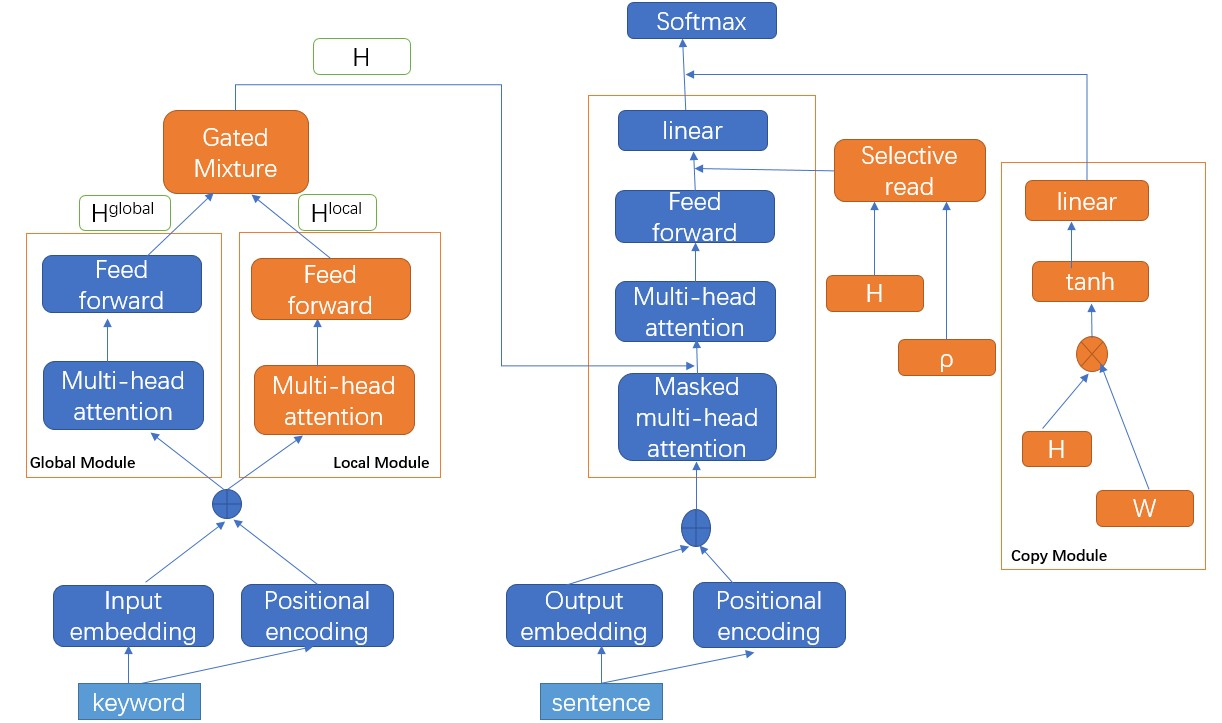
\includegraphics[width=12cm,height=8cm]{model2.jpg}
\caption{Global-Local-Copy Model}\label{fig:model}
\end{figure*}

\begin{equation}\label{equ:mixture}
    \mathbf{H} = \beta^s\mathbf{H}^{local} + (1-\beta^s)\mathbf{H}^{global}.
\end{equation}
Here, the scalar $\beta$ is a learned parameter between 0 and 1 that is specific to the scenario $s$.

\textbf{Decoder:} The copy module is in decoder module, the probability of generating any target word $y_t$, is given by the mixture of probabilities as follows

\begin{equation}\label{equ:mixture-prob}
    p(y_t) = p(y_t,g) + p(y_t,c)
\end{equation}

where $g$ stands for the generate-mode, and $c$ the
copy mode. the right of Fig.~\ref{fig:model} illustrates the copy module decoder. $H$ is global-local encoding the above-mentioned, $\zeta(y)$ is the weighted sum of hidden states $H$ corresponding to $y$, referred to as selective read in the right of Fig.~\ref{fig:model}. 

\begin{equation}\label{equ:zeta}
    \zeta(y) = \sum^{T}_{\tau = 1} \rho_\tau \textbf{h}_\tau 
\end{equation}

\begin{equation}\label{equ:rho}
    \rho_\tau = \left\{
        \begin{aligned}
        \frac{1}{K} p(x_\tau,\textbf{c}|\textbf{H}), \quad & x_\tau = y_t & \\
        0, \quad & otherwise &
        \end{aligned} 
        \right.
\end{equation}

where $K$ is equal to the number of positions with source keywords in the target sentence, $\tau$ is the index of source keywords, $T$ is the number of keywords, $t$ is the index of word in target sentence, and $p(x_\tau,\textbf{c}|\textbf{H})$ is the probability of the source keyword be copied in target sentence. 

The score of each mode is calculated:

\textbf{Generate-Mode}: first connect the output of the feed forward part of the transformer method and selective-read, and then $p(y_t,g)$ is calculated through the full connection. 

\textbf{Copy-Mode}: first calculate $\sigma(\textbf{H}\textbf{W})$, $\sigma$ is a non-linear activation function, here using the $tanh$ function. Next $p(y_t,c)$ is calculated through the full connection. 

\section{EXPERIMENTAL SETUP}\label{sec:experiment}
\subsection{Dataset}
In this paper,we focus on two sub-scenarios under the home: creative home and simple home. We select the description of the products in these two scenarios from the list of product recommendation reasons. We collected 150,743 sentences related to these products, after weak supervision, left 103,612 sentences. We chose sentences which keyword input only appears once as the test set. Training data format is shown in Tab.~\ref{table:format}. 

\begin{table}
\caption{Training data format }\label{table:format}
\begin{center}
\begin{tabular}{p{2.5cm}p{5cm}}
    \toprule
    Input & Output \\
    \midrule
    \begin{CJK*}{UTF8}{gbsn}
        创意,纸巾盒,欧式
    \end{CJK*} &
    \begin{CJK*}{UTF8}{gbsn}
        一款欧式风范榉木纸巾盒,盒身采用创意撞色设计,不仅能放杂物,还能作为桌面摆设,大中小三种尺寸可选,适合多种场合使用。
    \end{CJK*} \\
    \bottomrule
\end{tabular}
\end{center}
\end{table}

\subsection{Comparative Method}
%WWW这篇有一步寻找名词短语,我的替换方法是 形容词(1个或多个)+ 的 + 名词(0个或1个) 例如: 浪漫的荷花  这样子的词语
%None Phrase Selection部分,改成寻找【形容词(1个或多个)+ ‘的’ + 名词(0个或1个)】的短语,因为文中没有提到KeywordExpansion部分的k和None Phrase Selection部分的L取值,我就选了k=5和l=10,其他都和文中一样

\subsection{Training}
We take the words from source side of corpus as the input vocabulary and chose the words from target side of corpus which word frequency greater than 20 as the output vocabulary. The dimension of word embedding and hidden units are both 512,the minibatch was set to be 64. The parameter of global-local module $\beta$ is initialized by 0.5, the parameter $W$ in copy module is randomly initialized and the the parameter $p$ is initialized by zero.

\subsection{Evaluation}
There are no direct evaluation metrics so that evaluate text generation system is difficult.  We choose ROUGE \cite{lin2004rouge} and BLEU \cite{papineni2002bleu} metrics that are popularly used for generation tasks (especially Machine Translation and Summarization). These two metrics are both based on references, but there are thousands of ways to generate an appropriate sentence for a specific product,the limited references are impossible to cover all the correct results. So,we we use five evaluation standards for human evaluators to check the quality of the generated descriptions on a small test dataset of 30 instances. The manual evaluation metrics are listed in Tab.~\ref{table:evaluation}. The score of each manual evaluation metrics ranges from 0 to 5 with the higher score the better, see Tab.~\ref{table:evaluation-rule} for more detailed Grading Rules. All the generated sentences are evaluated by 5 experts and the rating scores are averaged as the final score.

\begin{table}
\caption{Manual Evaluation }\label{table:evaluation}
\begin{center}
\begin{tabular}{p{2.5cm}p{5cm}}
    \toprule
    Evaluation Metric & Description \\
    \midrule
    Fluency \cite{wang2016chinese} & Does the sentence read smoothly and fluently? \\
    Catchyness \cite{munigala2018persuaide} & Is the description attractive,catchy? \\
    Relatedness \cite{munigala2018persuaide} & Is the description semantically related to the target scene? \\
    Completeness & Is the description contains the corresponding scene, product and attribute? \\
    Informative & Is the description informative?\\
    \bottomrule
\end{tabular}
\end{center}
\end{table} 

\begin{table}
\caption{Manual Evaluation details}\label{table:evaluation-rule}
\begin{center}
\begin{tabular}{p{2.5cm}p{1cm}p{4.5cm}}
    \toprule
    Evaluation Metric & Score & Description \\
    \midrule
    \multirow{3}*{Fluency} & 0 & Not at all smooth \\
    ~ & 1-4 & how many places are not smooth minus how many points \\
    ~ & 5 & Very smooth\\
    \hline
    Catchyness & 0-5 & The ratio of attractive words in total words multiply by 5\\
    \hline
    \multirow{4}*{Relatedness} & 0 & Completely unrelated to the scene \\
    ~ & 1 & none \\
    ~ & 2 & Refer to the scene \\ 
    ~ & 3-5 & how many descriptions related to the scene, add how many points\\
    \hline
    \multirow{6}*{Completeness} & 0 & No input at all \\
    ~ & 1 & none \\
    ~ & 2 & Contains an input keyword \\ 
    ~ & 3 & Contains two input keyword\\
    ~ & 4 & There's no third word involved, but it's relevant\\
    ~ & 5 & Completely contains\\
    \hline
    \multirow{3}*{Informative} & 0 & No information at all \\
    ~ & 1 & It's describing the product \\
    ~ & 2-5 & how much information about the product, add how many points\\
    \bottomrule
\end{tabular}
\end{center}
\end{table} 

\subsection{Results}
We report the experimental results for our two approaches, i.e. global-local model and global-local-copy model. The difference between two models is former has no copy module. We compare our models with the Transformer method. Results are reported on the test data of 1472 instances, used for automatic evaluation and a held-out set of 32 instances, used for manual evaluation. The source keyword of test data for automatic evaluation are never appeared in train data. We choose the source keyword of test data that have scene name, product name and only one cpv value for manual evaluation.

From the perspective of considering our system as another machine translation system that converts some keywords of product(the scene name, product name, cpv data) into a persuasive product description with scene, we have results shown in Tab.~\ref{table:evaluation-automatic}. Popular machine translation and summarization metrics BLEU and ROUGE are used. There are four different ROUGE measures: ROUGE-N, ROUGE-L, ROUGE-W, and ROUGE-S, depending on the textual units to be compared. As can be seen from the results, our two methods are superior to Transformer in every indicator. Explain that both the global-local module and the copy module have a positive impact on the model. Because these two metrics are both based on references, and the copy module is aim to let the output sentence contain user-supplied input, so the results of global-local-copy model is better than global-local model.

\begin{table}
  \caption{Automatic Evaluation Metrics}
  \label{table:evaluation-automatic}
  \begin{tabular}{c c c c}
    \toprule
    Metrics & Transformer & Global-local & Global-local-copy\\
    \midrule
    ROUGE-1 & 0.3933 & 0.4050 & 0.4054\\
    ROUGE-2 & 0.1319 & 0.1446 & 0.1488\\
    ROUGE-3 & 0.0643 & 0.0740 & 0.0777\\
    ROUGE-4 & 0.0424 & 0.0514 & 0.0521\\
    ROUGE-L & 0.3259 & 0.3373 & 0.3423\\
    ROUGE-W & 0.1491 & 0.1552 & 0.1585\\
    ROUGE-S* & 0.1628 & 0.1762 & 0.1784\\
    BLEU-1 & 0.2964 & 0.3056 & 0.3096\\
    BLEU-2 & 0.1556 & 0.1671 & 0.1729\\
    BLEU-3 & 0.0807 & 0.0926 & 0.0977\\
    BLEU-4 & 0.0522 & 0.0632 & 0.0654\\
  \bottomrule
\end{tabular}
\end{table}

From the perspective of human psychology of persuasive product descriptions, we manually evaluated the generated descriptions using human evaluators. Five different measures were used to evaluate the human subjectiveness: Catchyness, Relatedness, Fluency, Completeness and Informative. It can be evidently observed in Tab.~\ref{table:evaluation-manual}. that the proposed system generated more catchy, better related, more fluency sentences compared to the Transformer method. Because our global-local module focuses on the description of the scene, resulting in the generated sentences with more descriptions of the scene, more appealing and more relevant to the scene. What's more, sentences generated by our model contain more input keywords and have more information about product.

\begin{table}
  \caption{Manual Evaluation Metrics}
  \label{table:evaluation-manual}
  \begin{tabular}{c c c c}
    \toprule
    Metrics & Transformer & Global-local & Global-local-copy\\
    \midrule
    Catchyness & 1.2235 & 1.2455 & 1.3320\\
    Relatedness & 2.4375 & 2.5000 & 2.7500\\
    Fluency & 3.4375 & 3.7187 & 3.9375\\
    Completeness & 3.6250 & 3.9375 & 3.9062\\
    Informative & 3.0312 & 3.4687 & 3.4687 \\
  \bottomrule
\end{tabular}
\end{table}

For qualitative analysis, we also provide the sentences generated from our system as well as other systems in the Tab.~\ref{table:case}. As we can see, the descriptions generated by our systems are competitive or better in terms of creativity, persuasiveness and fluency than the supervised baselines but have less overlap with the reference descriptions. This explains why our system is deemed to have underperformed than the baselines, as per the automatic evaluation scores. In general, the field of creative text generation demands looking beyond simplistic evaluation measures and it is about time that trainable metrics for evaluating persuasive text holistically, including aspects on creativity, coherency, novelty are proposed.

\begin{table*}
  \caption{Sample generations from different systems along with inputs and reference descriptions}
  \label{table:case}
  \begin{tabular}{p{2.5cm}p{12cm}}
    \hline
    Input & 
    \begin{CJK*}{UTF8}{gbsn}
        创意,挂钟,奢华
    \end{CJK*} \\
    Transformer & 
    \begin{CJK*}{UTF8}{gbsn}
        创意 十足 的 挂钟 , 舒适 静音 的 设计 , 温柔 的 花纹 , 灵动 而 神秘 , 让 你 爱 坐在 客厅 的 时光 里 里 静静 享受 质量 。
    \end{CJK*} \\
    Global-local & 
    \begin{CJK*}{UTF8}{gbsn}
        创意 挂钟 , 奢华 镶 钻 , 奢华 镶 钻 , 奢华 镶 钻 。
    \end{CJK*} \\
    Global-local-copy & 
    \begin{CJK*}{UTF8}{gbsn}
        创意 十足 的 大 号 挂钟 , 奢华 范 , 奢华 独特 。
    \end{CJK*} \\
    \hline
    Input & 
    \begin{CJK*}{UTF8}{gbsn}
        简约,挂钟,精致
    \end{CJK*} \\
    Transformer & 
    \begin{CJK*}{UTF8}{gbsn}
        简约 静音 挂钟 , 做工 精致 , 细节 精致 , 高档 品质 之选 。
    \end{CJK*} \\
    Global-local & 
    \begin{CJK*}{UTF8}{gbsn}
        可 摇摆 的 静音 挂钟 , 做工 精致 , 造型 独特 , 简约 大气 的 外形 符合 你 的 工作 品质 生活 , 静音 设计 , 增加 家中 的 灵动 性 。
    \end{CJK*} \\
    Global-local-copy & 
    \begin{CJK*}{UTF8}{gbsn}
        这 款 挂钟 , 造型 简约 大方 , 做工 精致 , 散发 着 大自然 的 气息 , 选用 的 静音 扫描 机芯 , 走时 准确 , 可 挂 在 墙上 , 方便 又 不 掉色 。
    \end{CJK*} \\
  \bottomrule
\end{tabular}
\end{table*}

\section{Conclusion}\label{sec:conclusion}

\section{Acknowledgments}

\bibliographystyle{ACM-Reference-Format}
\bibliography{refer}
\end{document}
